Figure \ref{fig:zonal_LEV_radius_Re200k} shows the radius of the LEV for different meshes at multiple phases.
Recall that LEV radius is considered to be
the radial distance from center of LEV core where maximum tangential velocity is achieved, and this tangential velocity is computed along multiple radial lines, and the peak tangential
velocity is obtained from this averaged tangential velocity along multiple radial lines.

M0\_nz50 mesh shows the largest radius among all the meshes. Mza1\_nz50 and Mza1\_nz100 show a similar radius.
Mza2\_nz50 shows the lowest radius among all the meshes, which is expected as mesh resolution is highest in this mesh, and as a result, a less diffused LEV is resolved.


\begin{figure}[H]
	\centering
	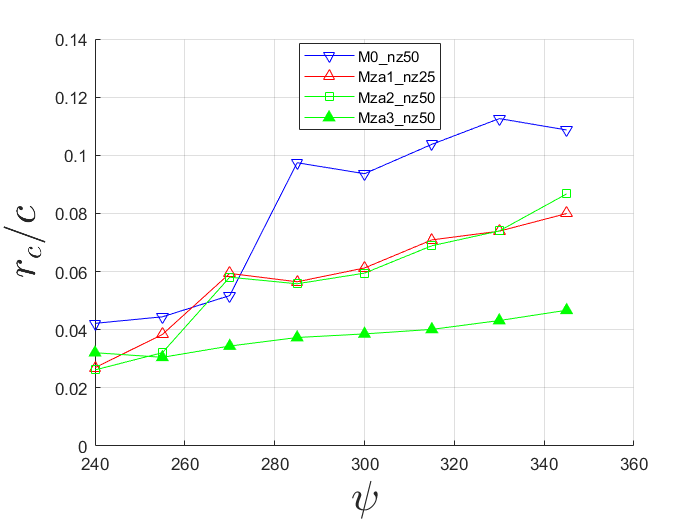
\includegraphics[width=0.7\textwidth]{figures/zonal_adapt_results/LEV_Re200k/LEV_radius_vp}
	\caption{ LEV radius for different meshes}
	\label{fig:zonal_LEV_radius_Re200k}
\end{figure}

Figure \ref{fig:zonal_LEV_location_Re200k} shows the location of the center of the LEV core for different phases after it is ejected from the airfoil surface.
Note that the LEV is ejected closer to the trailing edge as compared to the lower Reynolds number of $Re=40,000$, for the same advance ratio.
For all the meshes considered here, LEV shows a very similar path.

\begin{figure}[H]
	\centering
	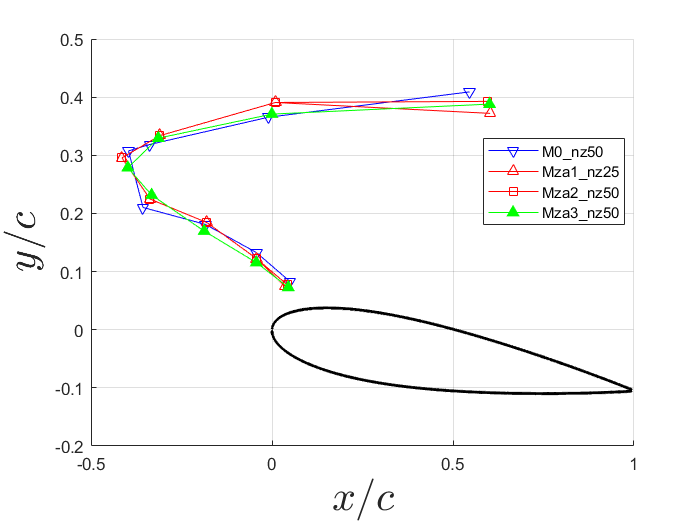
\includegraphics[width=0.75\textwidth]{figures/zonal_adapt_results/LEV_Re200k/LEV_location_Re200k}
	\caption{ LEV location for different meshes}
	\label{fig:zonal_LEV_location_Re200k}
\end{figure}
